% !TeX root = incremental_SS_Translation.tex
\chapter{Kalpasthāna: Introduction}

The \emph{Kalpasthāna} of the \emph{Compendium of Suśruta} is one of the most
important treatises on toxicology surviving from the ancient 
world.\footnote{\citet{liu-2021} provides a valuable overview of poison treatises 
in the ancient world, inexplicably omitting mention of the \emph{Kalpasthāna}.} 
Other treatises, such as the
\emph{\textgreek{θηριακά}} (\emph{On Beasts}) and
\emph{\textgreek{Ἀλεξίφαρμακα}} (\emph{Antidotes}) 
of Nicander of Colophon (fl.\ second century \BCE)
or the  
\emph{\textgreek{Περὶ τῶν ἰοβολῶν θηρίων καὶ δηλητηρίων φαρμάκων}} 
(\emph{On Venomous Beasts and Poisonous Drugs})
by Aelius Promotus (fl.\ ca.\ first century \BCE -- first century \CE)
do not approach the \emph{Kalpasthāna} in length, taxonomic detail or
organization.\footnote{On Aelius Promotus, see 
\cites[29]{smit-1870}[363--368]{gost-1897}{ihm-1995}. On
    Nicander, see \cite{gow-1953}, and the facsimile of \MS{Paris BNF Greek 
    suppl.\ 247} by \citet{touw-1997}.}

%\cite{Paris-suppl-247}

\section{The Sequence of Chapters}
\label{kalpa-chapter-sequence}

The Nepalese version of the \SS\ reverses the sequence of chapters 6 and 7.  

\begin{table}[h]
    \centering
     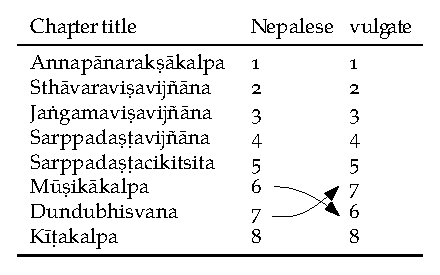
\includegraphics[width=0.65\linewidth]{chapters/media/kalpa}
%    \begin{tabular}{lll}
%    \emph{Chapter title} & \emph{Nepalese} & \emph{vulgate}   \\
%    \toprule
%      Annapānarakṣākalpa   &  1 &  1 \\
%     Sthāvaraviṣavijñāna & 2 &  2\\
%     Jaṅgamaviṣavijñāna &  3 & 3 \\
%     Sarppadaṣṭavijñāna & 4  &  4 \\
%     Sarppadaṣṭacikitsita & 5 & 5 \\
%     Mūṣikākalpa &  {6} & \textbf{7} \\
%     Dundubhisvana & {7} & \textbf{6} \\
%     Kīṭakalpa & 8 & 8 \\
%    \bottomrule  
%    \end{tabular}
\end{table}

% TODO: \usepackage{graphicx} required
%\begin{figure}
%    \centering
%    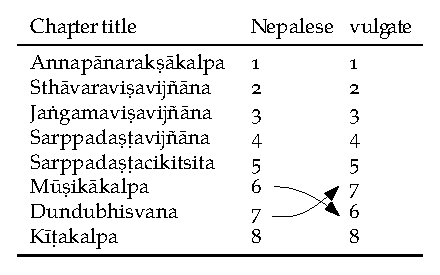
\includegraphics[width=0.65\linewidth]{chapters/media/kalpa}
%    \caption{}
%    \label{fig:kalpa}
%\end{figure}

\noindent
This difference in sequence does not have an immediately obvious 
significance, but it appears to be the most original known sequence of 
chapters, since it was already known to Jejjaṭa.\footnote{See note 
\ref{dalhana-rat-sequence} below.}

\section{The Spread of Indian Toxicological Lore to Medieval Islamic  
Authors}

The \SS\ was translated into Persian or Arabic at the Abbasid court in
the late eighth century by an Indian physician who is often known by
the name Mankah.\footnote{On the name and its variants, see
    \volcite{IB}[202, notes 2, 3]{meul-hist}.}  The principle source of
    information about this translation is the 
    \emph{`Uyūn al-anbā' fī ṭabaqāt al-aṭibbā} of Ibn Abī Uṣaybiʻah, Aḥmad ibn 
    al-Qāsim
    (1201--1270):\footnote{On `Abī
        Uṣayb`ia, see \cite{hill-2019}.}
\begin{quote}
    Mankah al-Hindī  was knowledgeable about the art of medicine,
skilled in treating disease, and moderate in his methods; a
philosopher of the previously mentioned group in the Indian
sciences. He was also conversant with the Sanskrit and Persian
languages: it was he who translated Shānāq’s \emph{On poisons}
from Sanskrit to Persian. Mankah was a contemporary of Hārūn
al-Rashīd, and during the latter’s caliphate he travelled from
India to Iraq, where he met with the caliph and treated 
him.\footnote{Translation from \volcite{3.2}[991--993]{sava-2019}.}
\end{quote}
`Abī Uṣayb`iah himself then went on to cite a passage that he relied on, taken 
from  
\emph{The History of the Caliphs and the Barmakids}  (\emph{Akhbār 
al-Barāmikah}) written by  Abū Ḥafṣ 
al-Kirmānī (fl.\ ca.\ 800).\footnote{This treatise is unfortunately lost to history and 
known only 
through citations in other authors.   See further, \cite{bosw-1994,blad-2011}.}


\volcite{IA}[352]{meul-hist}
\cite{lang-2018}

\citet[Introduction]{leve-1966} on 
\begin{itemize}
    \item translation of the \SS\ under the Barmakids (Pramukhas) in 
    eighth-ninth-century Baghdad:
    \begin{quote}
        Much more important is the fact
        that Mankah is known as the translator of the Susruta
        samhita, a huge medical compendium, for Yahya b.~Khalid. Ibn abi Usaibi'a 
        (1203/4--1270) also discussed
        Mankah as an important Indian physician. Al-Jaiz
        (d.\,868/9) knew of Mankah.'
        \ldots
        
        Yahya ibn Khalid, a Barmecide, was famous in his
        day in the field of science. In ibn al-Nadim, it is
        related that Yah.ya sent a scholar to India to study
        Indian drugs and religion, and brought Indian physi-
        cians and philosophers westward so that he might learn
        from them.
        Caliph al-Ma'mfin  also was interested in the sci-
        ences and so brought many scientists to his court from
        Jundishapfir where there were not only Greek men of
        science but also Indians who had brought their science
        and wisdom.\footnote{\cite[6]{leve-1966}}
    \end{quote}
    
    \item ibn Wahshiya's Book on Poisons (ca. 950). 
    \begin{quote}
        Not much is known of Shanaq himself. However,
        what is one of the earliest mentions of him is made in
        ibn Wahshiya's Book on Poisons (ca.\ 950). He refers
        to Shanaq's book as great and important. This state-
        ment is attested to by the fact that much of Shanaq's
        work was used by ibn Wahshiya. It was not, however,
        a base upon which the latter's work was built, as
        Strauss has claimed.\footnote{Idem.}
    \end{quote}
    \item The Poison book of Cāṇakya.\footcite{stra-1934}

\item The Poison Book of Maimonides (ca.\,1198 \CE):

\citetitle{rosn-1968},\footcite{rosn-1968}  was written in
approximately July 1198 at the request of his patron, al-Qadi
al-Fadil (1135--1200) who served in Cairo under the Fatimid and
Ayyubid administrations.\footcite[31]{krae-2005}
\end{itemize}
